
\section{Microcontrolador e IDE} \label{microcontrolador_ide}

\subsection{Microcontrolador}

Microcontroladores são circuitos integrados compactos desenvolvidos para governar
uma operação específica em um sistema embarcado. No contexto da aplicação deste
trabalho, o uso de um microcontrolador é fundamental para se obter o controle
desejado de trajetória e posicionamento do robô.

Duas placas de microcontrolador o BluePill e ESP32 Devkit v1 foram testadas.
Ambas possuem processadores de 32bits e podem ser alimentadas através dos pinos
de 5V e 3.3V, e também através do connector micro-USB-B.

A escolha dessas placas foi motivada pelo seu custo de aquisição e pelos
componentes e opções de comunicação disponíveis. A placa BluePill já havia sido
adquirida anteriormente ao desenvolvimento deste projeto, de modo que seu uso
não incorreria em custos adicionais. Semelhantemente, a escolha da placa ESP32
Devkit V1 também foi motivada também pelo custo, mas a capacidade de integração
por Bluetooth mostrou-se particularmente relevante neste contexto, tornando a
placa uma boa candidata para esta aplicação. Tal integração integração será
discutida nas seções a seguir.

A \autoref{precos_placas} compara a faixa de preço entre as principais
placas de desenvolvimento disponíveis para compra em território nacional.

\begin{table}[ht]
	\centering
	\caption{Comparação de preços entre as placas de desenvolvimento}
	 \begin{tabular}{|c|c|}
		\hline
		\textbf{Placa de desenvolvimento} & \textbf{Faixa de preço em R\$} \\ \hline
		BluePill (STM32F103C8T6) &  23 - 49 (já adquirido anteriormente) \\ \hline
		ESP32 DevKit V1  &  40 - 80   \\ \hline
		Arduino Due R3 &  320 - 470   \\ \hline
		Nodemcu v3 ESP8266 & 22 - 35   \\ \hline
		Raspberry pi pico (1, 2, W, H)  & 36 - 66  \\ \hline
	\end{tabular}
	\fonte{Própria}
	\label{precos_placas}
\end{table}

Os preços aqui apresentados têm como base os valores praticados pelas principais
lojas nacionais de componentes eletrônicos online:
\begin{itemize}
	\item https://www.rsrobotica.com.br/
	\item https://www.robocore.net/
	\item https://www.makerhero.com/
	\item https://www.iot-robotica.com.br/
	\item https://www.ardurobotica.com.br/
	\item https://curtocircuito.com.br/
	\item https://www.saravati.com.br/
	\item https://www.a2robotics.com.br/
	\item https://www.ardurobotica.com.br/
	\item https://www.casadarobotica.com/
\end{itemize}



\subsubsection{BluePill - STM32F103C8} \label{STM32_referencia}

A placa BluePill embarca o microcontrolador STM32F103C8.
``STM32'' é uma família de microcontroladores de 32-bits fabricados pela
ST-Microelectronics. O processador empregado nessa família é o ARM Cortex-M3
\cite{cortex_m3}, baseado em arquitetura Harvard, com 64Kbs de memória flash.

De acordo com o livro \textit{Discovering the STM32 Microcontroller}
\cite{stm_doc} e a documentação colaborativa do projeto STM32-base.org
\cite{stm32_base_org}, a placa possui também 7 timers, 2 ADCs, e 9 interfaces de
comunicação, incluindo I2C,  USART, SPI, e USB 2.0.

A placa STM32 apresenta 7 pinos que suportam canais de PWM de 5V, e outros 8
canais de 3.3V, e pode ser alimentada via microUSB de 5V. Existem 3 grupos de
pinos: $P_{A}$, $P_{B}$ e $P_{C}$. Os pinos $P_{A}$ vão de $P_{A0}$ 
a $P_{A15}$, os $P_{B}$ vão de $P_{B0}$ a $P_{B15}$, e $P_{C}$, com apenas 3
pinos, de $P_{C13}$, $P_{C14}$ e $P_{C15}$.
A relação geral dos pinos pode ser melhor observada na figura 
\autoref{stm32f103c8_pinout}.

\begin{figure}[ht]
	\centering
	\caption{Diagrama de pinos do STM32F103C8}
	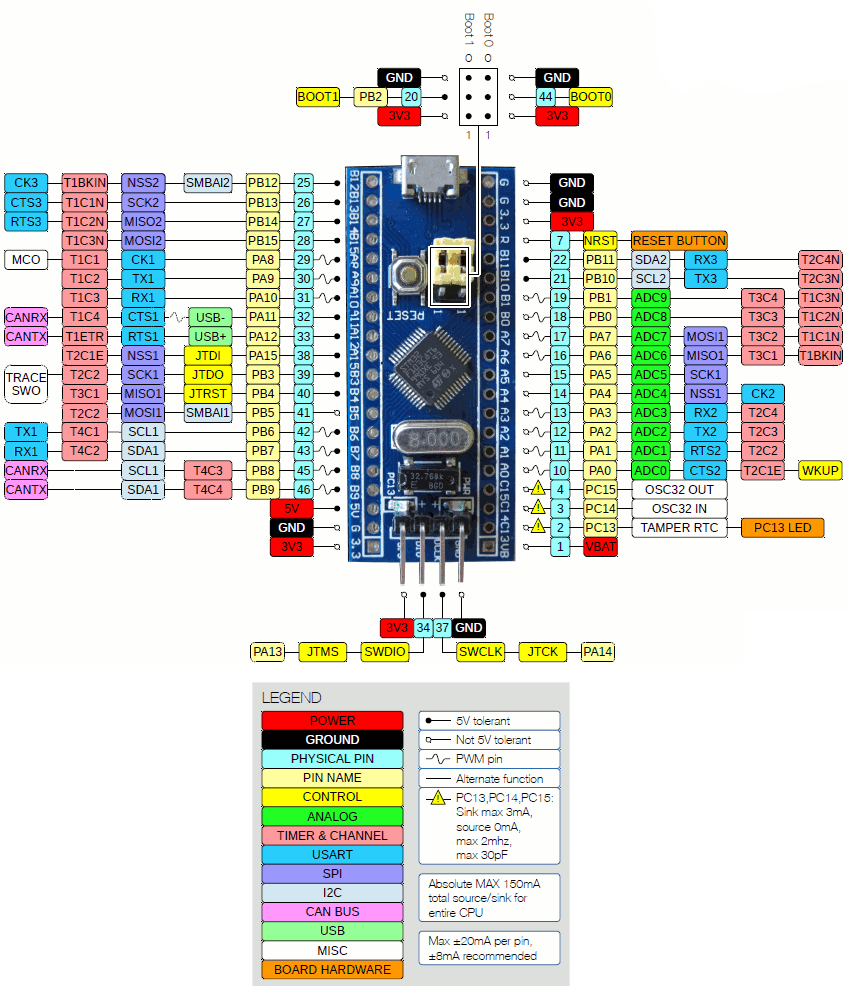
\includegraphics[width=1.0\textwidth]{figures/stm32f1_pinout}
	\fonte{\cite{apostila_microprossados}}
    \label{stm32f103c8_pinout}
\end{figure}

O gravador ST-LINK V2 é o padrão para carregar projetos no microcontrolador.
Esse gravador, cuja versão original (\autoref{stlinkv2_original}) é fabricada
pela ST-Microelectronics, pode ser encontrada em uma versão paralela a menores
custos online (\autoref{stlinkv2_cheap}). Contudo, as versões paralelas, por
serem produzidas por fabricantes diversos, e por vezes não claramente indicados 
na descrição do produto. Por essa razão, pode haver variação na relação de
pinos (\autoref{stlinkv2_cheap_pin_diff}).

É possível modificar o firmware da placa STM32F103C8 para permitir o
carregamento de projetos via USB, contudo tal esse procedimento
é nativamente suportado ST-Microelectronics, tornando necessário o uso de
ferramentas de terceiros - por vezes, mesmo projetos de código aberto não mais
ativamente mantidos \cite{stm32duino_bootloader}.
A conexão micro-USB-B ainda funciona como uma comunicação serial, podendo ser
usada como uma porta serial para fins de \textit{debugging}. Contudo, utilizá-la
ao mesmo tempo que o ST-link pode danificar o microcontrolador, já que o
regulador recebe 5V da entrada USB e disponibiliza 3.3V volts, ao mesmo tempo
em que mas 3.3V também estão sendo disponibilizados diretamente a partir do
gravador ST-link.

\begin{figure}[ht]
	\centering
	\caption{St-Link V2 original}
	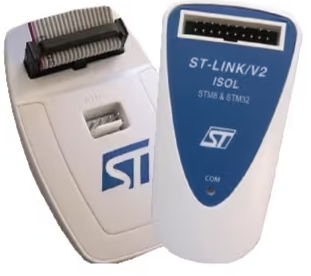
\includegraphics[width=0.5\textwidth]{figures/stlinkv2_original}	
	\fonte{\cite{st_link_v2}}
    \label{stlinkv2_original}
\end{figure}


\begin{figure}[ht]
	\centering
	\caption{St-Link V2 paralelo}
	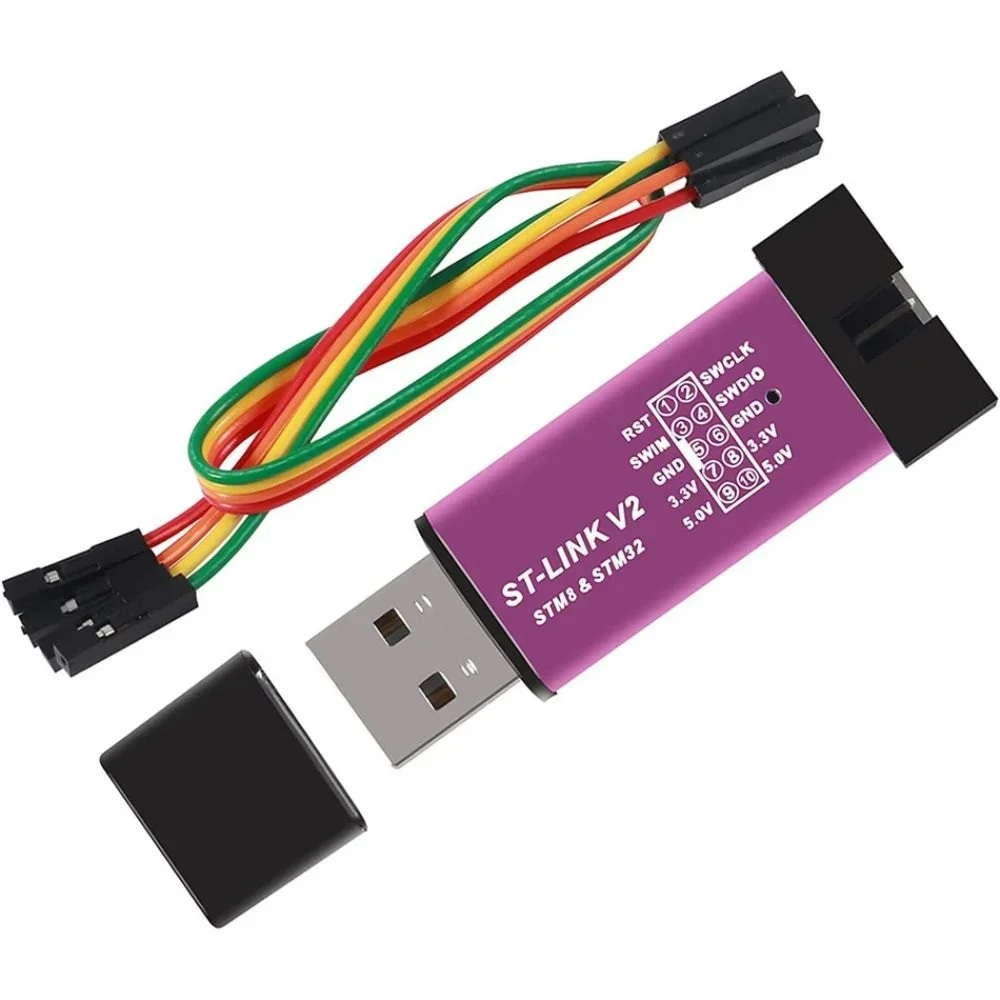
\includegraphics[width=0.5\textwidth]{figures/stlinkv2_cheap}	
	\fonte{\cite{stlinkv2_cheap_ref}}
    \label{stlinkv2_cheap}
\end{figure}


\begin{figure}[ht]
	\centering
	\caption{St-Link V2 paralelo e pinos despadronizados}
	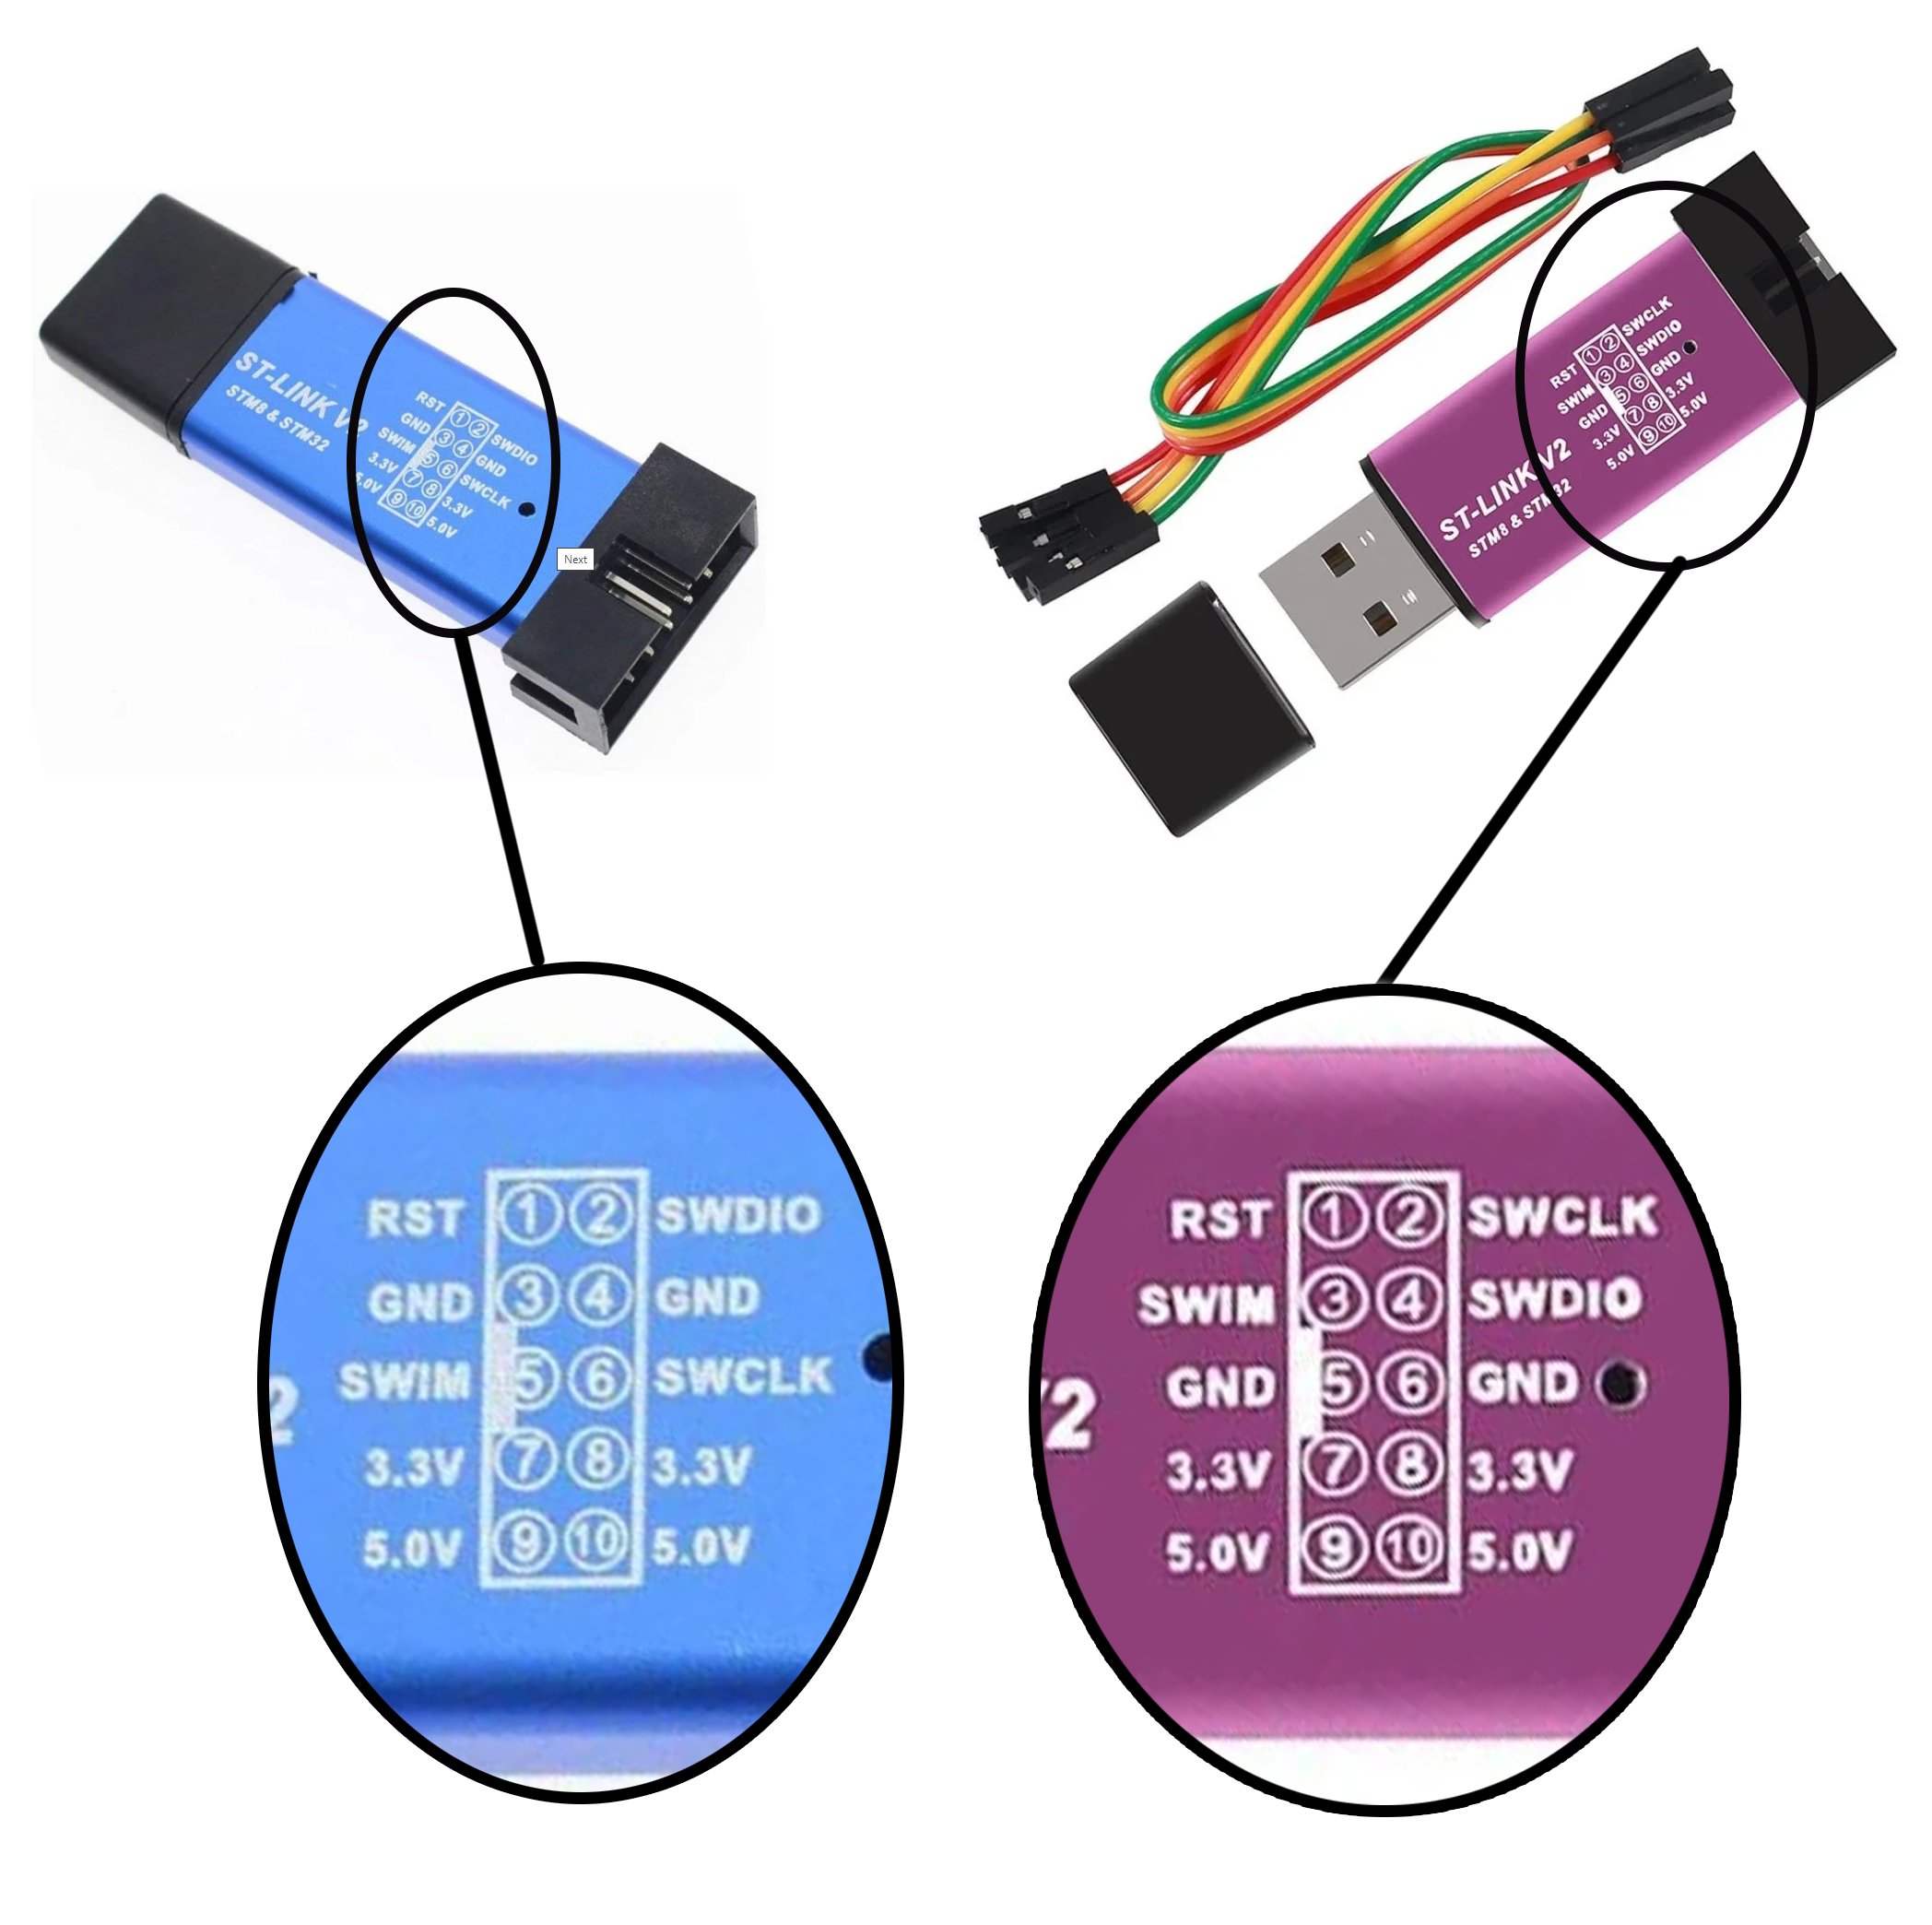
\includegraphics[width=0.5\textwidth]{figures/stlinkv2_cheap_pin_diff}
	\fonte{Adaptado de \cite{stlinkv2_cheap_ref,stlinkv2_cheap_pin_diff_ref}}
    \label{stlinkv2_cheap_pin_diff}
\end{figure}

No restante desse trabalho, todas as menções a ``STM32'' referem-se à placa
BluePill.


\subsubsection{ESP32 Devkit v1} \label{ESP32_referencia}

A placa ESP32 Devkit v1, de fabricação da DOIT.am, possui o microcontrolador
ESP32-WROOM-32E (\autoref{esp32_pinout}), fabricado pela Espressif Systems.
A série ESP32 foi lançada em 2016 \cite{anuncio_esp32}, e possui arquitetura de
32 bits. Ela tem se tornado popular por possuir opções com integração Bluetooth
e WiFi. O microcontrolador ESP32-WROOM-32E possui um processador dual core
ESP32-D0WD-V3 \cite{esp32_wroom_32e_datasheet}, com frequência máxima de 240MHz,
WiFi 2.4Ghz de até 150Mbps e Bluetooth 4.2. Embora a placa tenha 48 GPIOs, elas
estão endereçadas em apenas 25 pinos. Entre os periféricos, existem 15 canais
ADC, 2 interfaces UART, 2 canais DAC, 25 PWM, uma interface de SPI, I2C e I2S,
e 9 interfaces de toque capacitivo
\cite{esp32_reference_2,esp32_reference}.

\begin{figure}[ht]
	\centering
	\caption{Diagrama de pinos da placa ESP32 Devkit v1}
	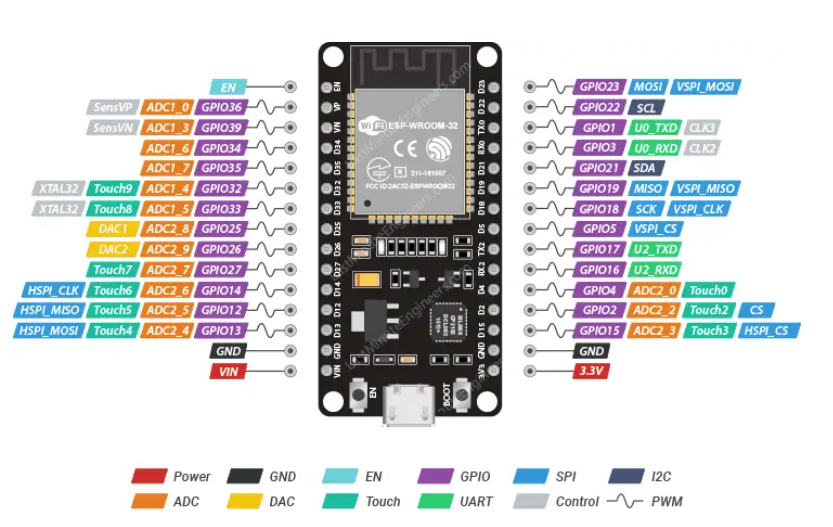
\includegraphics[width=1.0\textwidth]{figures/esp32_pinout}
	\fonte{Adaptado \cite{esp32_reference}}
	\label{esp32_pinout}
\end{figure}

Artigos contribuídos pela comunidade online sobre a placa ESP32 Devkit v1 
\cite{esp32_reference_2,esp32_reference} sugerem que nem todos os 25
pinos podem ser livremente utilizados - alguns possuem limitações de uso de
acordo com o periférico em uso. A \autoref{esp32_pinout_ref} resume as
recomendações de uso do pinos. Diferentemente da placa STM32, é possível
carregar projetos na placa ESP32 Devkit v1 nativamente via USB.

\begin{figure}[ht]
	\centering
	\caption{Recomendação de uso dos pinos da placa ESP32 Devkit v1}
	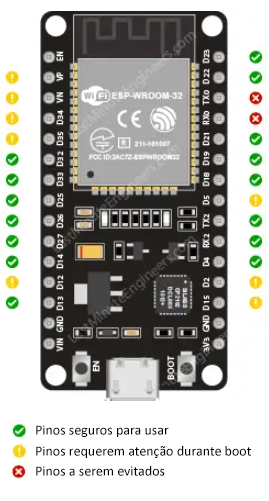
\includegraphics[width=0.35\textwidth]{figures/esp32_pinout_ref}
	\fonte{Adaptado \cite{esp32_reference}}
	\label{esp32_pinout_ref}
\end{figure}

No restante deste trabalho, todas as menções a ``ESP32'' referem-se à placa
ESP32 Devkit v1.


\subsection{IDE}

\subsubsection{Atollic TrueSTUDIO}

\begin{figure}[ht]
	\centering
	\caption{Interface Atollic}
	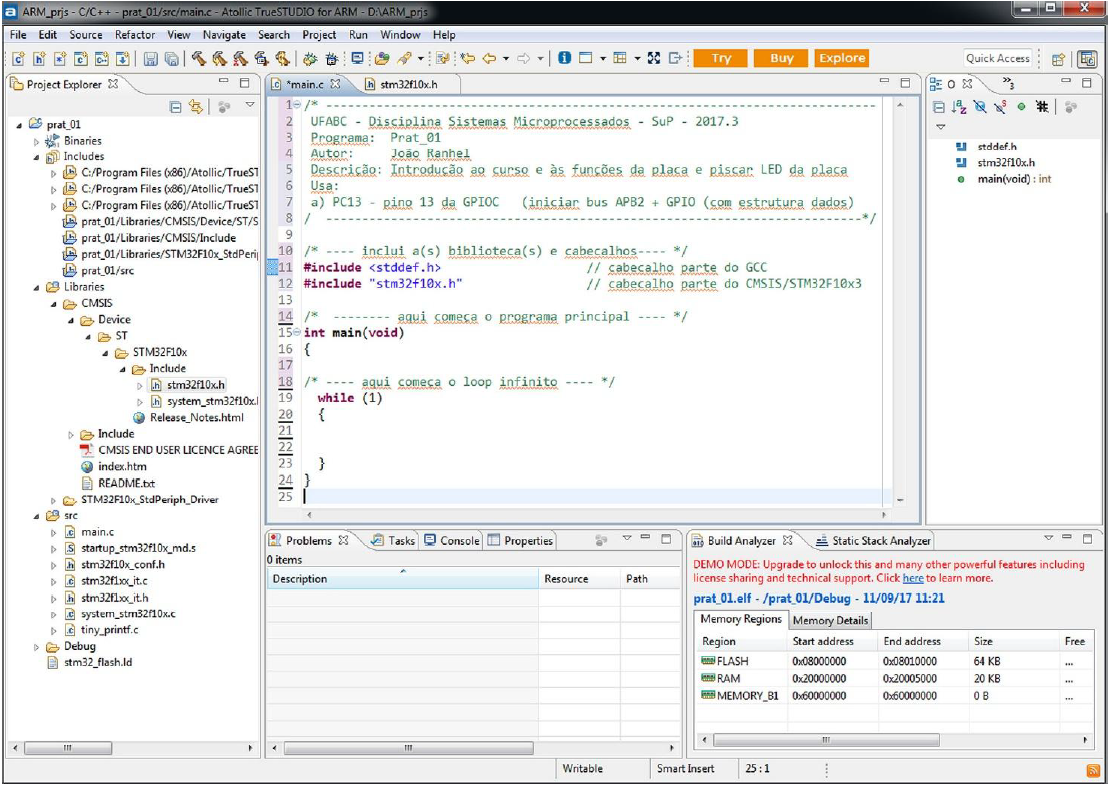
\includegraphics[width=0.8\textwidth]{figures/atollic}
	\fonte{\cite{apostila_microprossados}}
\end{figure}

A IDE padrão empregada para programar projetos para a placa STM32 é o TrueSTUDIO,
distribuído pela Atollic, que foi adquirida pela ST-Microelectronics em 2017.
Trata-se de um software livre para programar em C/C++, criado com base na
plataforma Eclipse, e que possui todas as funções necessárias para o
desenvolvimento com a placa STM32, tais como edição, compilação e debugging.
Uma de seus principais vantagens é a ausência de limitações quanto ao tamanho
do projeto, o que o torna ideal para trabalhos profissionais. A IDE TrueSTUDIO
deixou de receber atualizações em 2017, depois da aquisição da Atollic pela 
ST-Microelectronics \cite{apostila_microprossados}.


\subsubsection{Arduino IDE}

Criado para ser a IDE das placa de desenvolvimento Arduino, a primeira
versão da Arduino IDE foi criada em 2005 \cite{arduino_id_history}.
Suas versões mais populares disponíveis para o público são 1.0.6 e 1.8. 
A versão 1.8 foi lançada em 2016 e recebeu atualizações até 2021, 
e a versão 2.0.0 foi lançada em 2022 \cite{arduino_tag_2}.

\begin{figure}[ht]
	\centering
	\caption{Interface Arduino}
	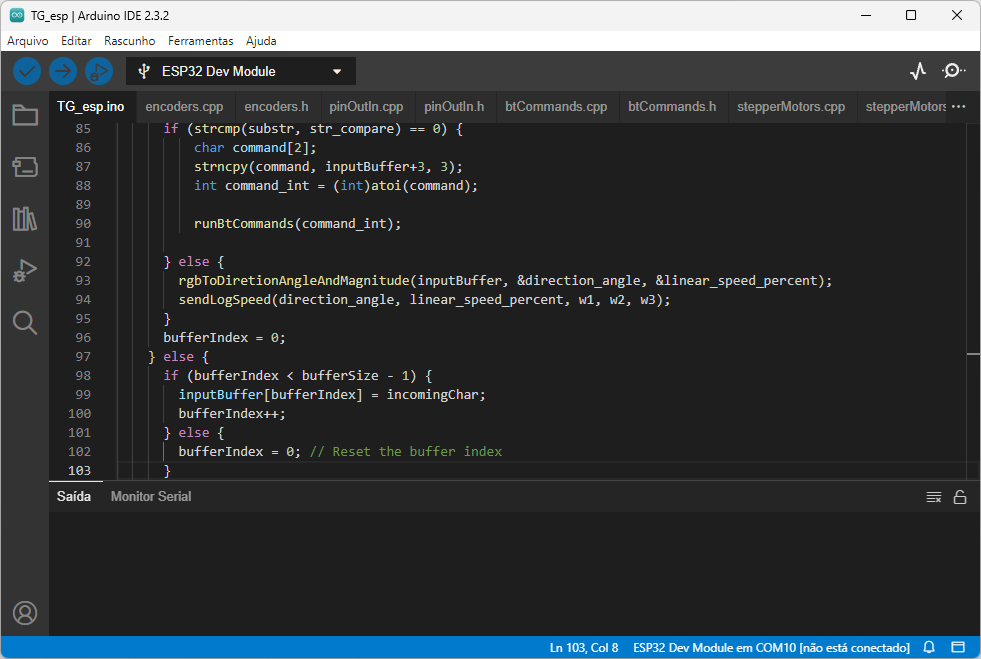
\includegraphics[width=0.9\textwidth]{figures/arduino}
	\fonte{Própria}
\end{figure}

\subsection{Escolha do microcontrolador e IDE}

\subsubsection{IDE}

Devido a complicações nas configurações de múltiplas saídas de PWM com o 
TrueSTUDIO, optou-se por usar Arduino como alternativa. Um obstáculo a essa
alternativa é que o Arduino não é compatível com STM32 nativamente. Esse
empecilho pode ser contornado por meio do uso do projeto Arduino\_STM32
\cite{arduino_stm32}, de Roger Clark. O projeto contem os arquivos na linguagem
C necessários para viabilizar o uso do hardware da placa STM32 com a Arduino IDE.
Até o momento de escrita deste trabalho, o projeto era compatível apenas com a
versão 1.8 da Arduino IDE.

Transposto o obstáculo inicial à sua utilização, a Arduino IDE do Arduino 
logo se demonstrou uma opção mais viável e flexível, tanto pela vasta lista
bibliotecas disponibilizadas por contribuidores voluntários quanto pela grande
quantidade de documentações de projetos independentes.

A Arduino IDE também é compatível com a placa ESP32 por meio do uso da
biblioteca arduino-esp32 \cite{arduino_esp32}, disponibilizada e mantida
pela Espressif Systems.

\subsubsection{Microcontrolador}

Durante o desenvolvimento deste projeto, algumas dificuldades tornaram a
utilização da placa STM32 inviável. Entre esses dificuldades, destacam-se a
impossibilidade do uso da porta micro-USB-B da placa STM32 simultaneamente ao
gravador ST-link, bem como a impossibilidade de se manter o módulo HC-05 ligado
durante o processo de gravação na placa. Esta última dificuldade ocasionou a
perda de dois módulos HC-05, dado que, no tocante aos pinos de comunicação serial,
quaisquer comportamentos diferentes do padrão durante a gravação de um podem
ocasionar dano ao módulo (o que de fato ocorreu, uma vez que o módulo HC-05 foi
deixado conectado à placa STM32 durante a gravação múltiplas vezes), e aquela
foi causa de dano à própria placa STM32.

Tais dificuldades no uso da placa STM32 com relação à conexão via micro-USB-B e
o uso do módulo HC-05 demonstraram que a placa ESP32 era uma melhor candidata 
para uso neste trabalho. A troca de placas não acarretou mudanças significativas
em outras partes do projeto, dado que a placa ESP32 apresenta integração
com Bluetooth nativamente e suporta gravação de projetos via micro-USB-B
para gravação ao mesmo tempo em que a comunicação serial é utilizada para
\textit{debugging}, e também que foi possível continuar a utilizar a Arduino IDE
por meio da biblioteca arduino-esp32.